\section{Moravec}\label{sec:moravec}
Moravecs hjørne detektor\cite{moravec}, er en af de tidligste feature detektorer, og definere et interessepunkt, som værende et hjørne. Moravec anvender denne definition til at opnå en matematisk formulering af hjørner ved at bruge et dataindsamlingsvinduer på 3x3, 5x5 eller 7x7 pixel regioner. De interessepunkter findes når auto-korrelationen imellem de forskudte billeder er stor. Dataindsamlingsvinduet kan bruges til at detektere hjørner, ved at forskyde  dette med én pixel i alle principielle retninger (horisontalt, vertikalt og diagonalt) og udregne intensitetsvariationen. Denne variation kan beskrives med en vægtet funktion over vinduet  \emph{(MSSD: Mean Summed Square Difference)}, der udregner forskellen på vinduerne:
\begin{equation}
E(u,v)= \sum_{\forall \text{x,y i dataindsamlingsvinduet}} w(x,y)[I(x+u,y+v) - I(x,y)]^2
\label{moravec}     
\end{equation}
hvor $(u,v)\in \lbrace -1,0,1 \rbrace$ er forskydningen af vinduet, der summere over alle pixels i dataindsamlingsvinduet $w$, der har centrum i $(x,y)$. Den mindste forskel i de otte skift, definere punktets \textit{hjørnestyrke}.
$$
C(x,y)=min(E(u,v))
$$
Minimum af $E$ er interessant, fordi den kan identificere, om et naboområde er identisk med det original område, og derved afgøre, om punktet er et hjørne. Der opstilles en grænseværdi for $C$, der bestemmer mindsteværdien for et hjørne. Figur \ref{fig:moravec} illustrere en udregning af $MSSD$ af et diagonalt skift på en isoleret sort pixel (med en intensitet på 0) på en hvid baggrund (med en intensitet på 255) og på et idealt hjørne. Det røde vindue indikere det originale vindue og det blå indikere  vinduet forskudt med vektoren i retnignen $(1,-1)$. 
\begin{figure}[H]
    \centering
    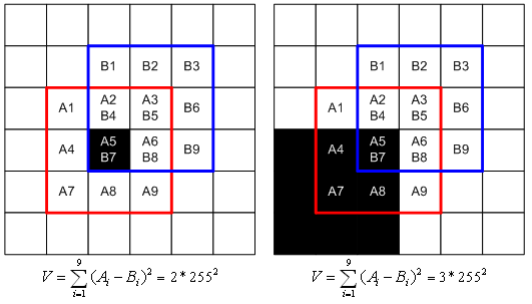
\includegraphics[width=0.45\textwidth]{fig/25.png}
     \vspace{-1em}
    \begin{center}    
       \caption{\textcolor{gray}{\footnotesize \textit{ WSSD udregninger for intensitetsvariationer imellem forskudte vindue. }}}
    \label{fig:moravec}
     \end{center}
     \vspace{-2.5em}
  \end{figure} \noindent
Moravec lider af følgende problemer pga. dens simplicitet. 
\begin{itemize}
\item{Der undersøges kun et diskret sæt af pixelskift (i hver principiel retning) og resultatet er derfor anisotropisk, hvilket vil sige afhængig af retning. Undersøges en kant, der ikke er horisontal, vertikal eller diagonal, vil den mindste intensitetsvariation være stor, og derved kan punktet fejlagtigt detekteres som et hjørne.}
\item{Det skiftende vindue er rektangulært, og metoden er derfor meget følsom overfor støj i billedet.}
\item{Detektoren finder punkter lokaliseret på kanter. Små deformationer i kanterne som støj, vil resultere i at den mindste intensitetsvariation vil være relativt stor, og derfor detektere punktet som værende et interessepunkt.}
\end{itemize}
% <evt konklusion>
% <måske billeder download cornerdetection.pdf>
\subsection*{Moravec(I)}
\begin{enumerate}
\item{For hvert pixel i billedet, udregnes auto-korrelationen imellem skift af $(x,y) \in [-1,0,1]$. udregnet ved ligning \ref{moravec}}
\item{\textit{"Hjørnestyrken"} udregnes for hvert pixel ved at finde $C(x,y)=min(E(u,v))$}
\item{En grænseværdi sættes sættes for $C(x,y)$, og værdier i punkter, der er større end grænseværdien, returneres}
\end{enumerate}
\subsection*{Konklusion}
Moravec er som nævnt en simpel algoritme, med mange udfordringer, der gør at den ikke bruges som en repeterbar detektor. Detektoren er i dag ikke i sig selv relevant, som den var da den blev udgivet, men bygges videre på i andre detektorer, f.eks. \cite{Harris} beskrevet i sektion, \ref{sec:harris} som direkte tilgår de nævne problemstillinger med Moravec.